\documentclass{article}
\usepackage[utf8]{inputenc}
\usepackage{amsmath}
\usepackage{graphicx}
\usepackage[a4paper, total={6in, 10in}]{geometry}
\usepackage{float}
\usepackage{caption}
\usepackage{hyperref}
\usepackage{subcaption}
\newcommand{\xdashrightarrow}[2][]{\ext@arrow 0359\rightarrowfill@@{#1}{#2}}
\usepackage{comment}

\title{Big data 1}
\author{Anton Rosenberg}
\date{May 2022}

\begin{document}

\maketitle
\newpage
\section{a}
\subsection{Results}
The three classifiers I chose to implement were Random forest, SVM with Rbf kernel and Logistic regression with liblinear solver. Using these three methods stratisfied K fold was used with 5 folds to fit the hyper parameters for the SVM and Logistic regression model. Furthermore the entire process was run 100 times (monte carlo simulation) and the final scores were the mean of the scores during these runs see table \ref{score}. The data was also split into train and test data at the start of each run were the score was taken on the test data after being fitted and its hyper parameters tuned on training. The score is around 80\% for all the classifiers with a relatively small standard deviation which would indicate that the data are quite separable bot not linearly. This was concludeed since if it were an SVM model with linear kernel should achieve an accuracy of 100\% which it did not since it preformed worse than the rfb kernel used with only an accuracy of about 0.74 with std of 0.06. The only data prepossessing made was to normalise the data so that all features have values between 0 and 1. Finally a record of the images which were classified incorrectly was kept during the 100 runs and can be seen in figure \ref{wrong}, here the x-axis represents the picture number and the y-axis the number of times that picture was incorrectly classified. 

From the scores we can see that the SVM model preforms better than the others this could be due to the fact that SVM works well when we don't know alot about the data and how it's distributed which is the case for the images in the CATSnDOGS data set. However SVM is also usually prone to overfitting when using a complex kernel on a data set where the feature number is vastly larger than the number of samples hence it's surprising that the model preformed so well on the test set. As for the kernel chosen it's difficult to know which one to use through trial and error the default rfb was found to work best. It's surprising that the logistic regression model worked so well since we have a lot less samples than features and we haven't done any feature reduction. This could be due to the fact that the l2 penalisation was used to minimize the negative effect of having less samples than features. When looking at the difference between classifying dogs and cats we look at the TPR which is the rate at which dogs are correctly classified and the TNR the same for the cats. We can see that the models have roughly the same amount of errors for both the dogs and the cats which would indicate that they are equally difficult to predict. When looking at the images which were consistently mislabeled there were a few which pictures which were incorrectly classified all the time by all classifiers. One example of these pictures can be seen in \ref{faulty data}. Here we see that the image clearly is of a cat but the label says it's a dog so we have some incorrectly labeled pictures in our data set which explains why they are incorrectly classified. There are probably some pictures which are outliers as well which would make them difficult to classify correctly for example a dog with very catlike features. 
\subsection{Conclusion}
As a conclusion we can say that it's difficult to separate dogs from cats completely but it can be done quite successfully since an accuracy of around 80\% was achivable. Furthermore the misslabeled data further increases the difficulty for a classifier to achieve good scores and they are consistently miss labeled by all three classifiers tested. The dogs and cats seem to be equaly hard to classify from the TPR and TNR for all the models.  
\begin{table}[H]
    \centering
    \begin{tabular}{c|c|c|c|c}
        Model & accuracy & std & TPR & TNR \\
         SVM & 0.81 & 0.056 & 0.82 & 0.81 \\
         Random forest & 0.78 & 0.065 & 0.79 & 0.76 \\
         Logistic regression & 0.77 & 0.057 & 0.761 & 0.79
    \end{tabular}
    \caption{Scores for the different models}
    \label{score}
\end{table}
\begin{figure}[ht]
\begin{subfigure}{.33\textwidth}
  \centering
  % include first image
  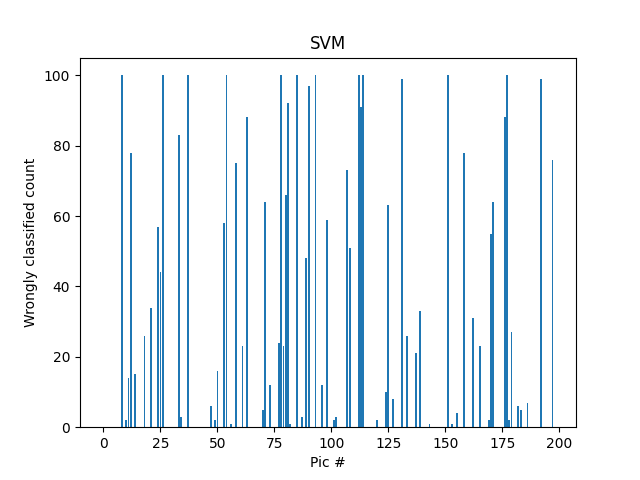
\includegraphics[width=1\linewidth]{1a/SVM.png}  
  \caption{Put your sub-caption here}
  \label{fig:sub-first}
\end{subfigure}
\begin{subfigure}{.33\textwidth}
  \centering
  % include second image
  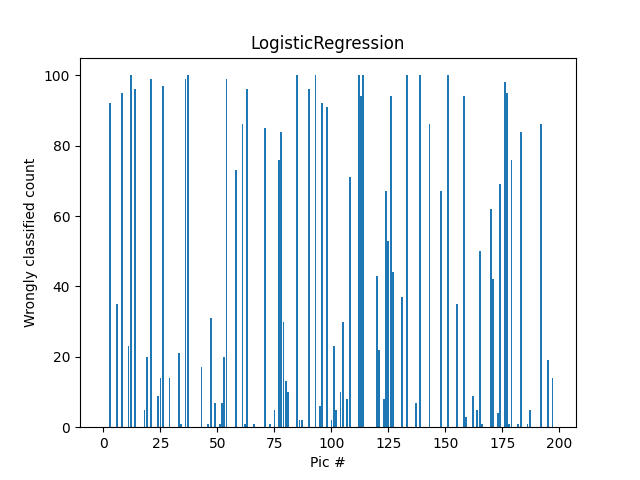
\includegraphics[width=1\linewidth]{1a/Logistic regression.png}  
  \caption{Put your sub-caption here}
  \label{fig:sub-second}
\end{subfigure}
\begin{subfigure}{.33\textwidth}
  \centering
  % include second image
  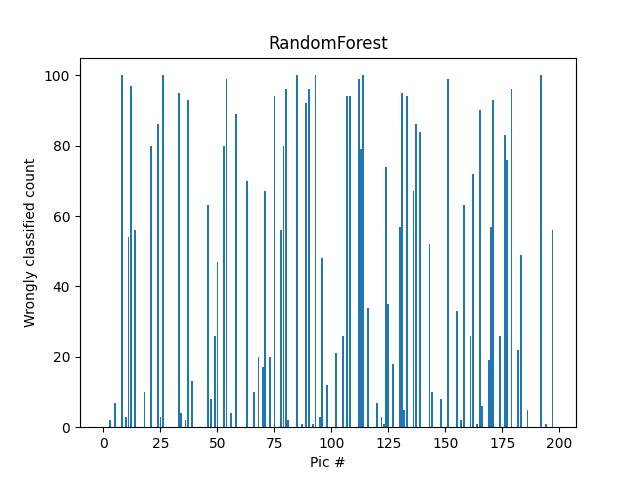
\includegraphics[width=1\linewidth]{1a/Random Forest.png}  
  \caption{Put your sub-caption here}
  \label{fig:sub-second}
\end{subfigure}
\caption{Put your caption here}
\label{wrong}
\end{figure}
\begin{figure}[H]
    \centering
    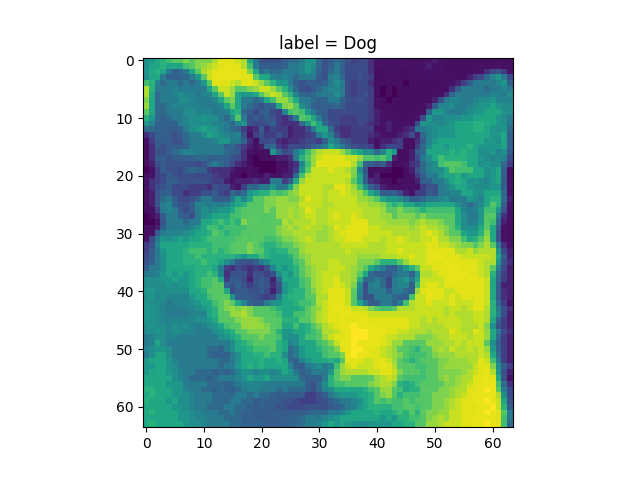
\includegraphics[scale=0.5]{1a/Dirty data.png}
    \caption{Faulty data}
    \label{faulty data}
\end{figure}
\newpage
\section{b}
\subsection{Result}
The three different classification methods used for finding the most important features were Logistic regression, Random Forest and SVM with linear kernal. Bootstrapping was used 100 times to see which features were selected with high certainty the results for each method can be seen in figure \ref{imp feat} and figure \ref{imp pixels}. We can see that Random forrest clearly looks at the pixels around the forhead, eyes and nose of the cats and dogs \ref{RandF}. We can also see from figure \ref{RandForSel} that the model is not very certain on its feature selections since few of them were selected above 40\% of the time. As for the SVM method it's difficult to see why these pixels are deemed important since they don't cluster around any paricular area of the picture like the around the eyes for example but rather seem to be cluster of pixels around the entire picture. This could be because the linear kernal is poorly suited for this data set this could also be why so few pixels were selected above the threshold of 60\%. The logistic regression also deemed a lot of pixels as important and alot of the features were selected 100\% of the time compared to the Random forest hence logistic regression and SVM seems to be more certain in their feature selection.  The stability of the chosen pixels is improved vastly by bootstrapping and choosing a threshold were only features selected more than the threshold are kept. The threshold was set at 60\% for the pixels shown in \ref{imp pixels}.
\subsection{Conclusions}
Logistic regression and SVM seems to be the most robust when it comes to certainty in feature selection, they also looks at a lot more features than the Random Forest model. Random forest seems to have trouble deciding which features are deemed important and zero of the features were selected 100\% of the time in the bootstrapping. 
\begin{figure}[ht]
\begin{subfigure}{.33\textwidth}
  \centering
  % include first image
  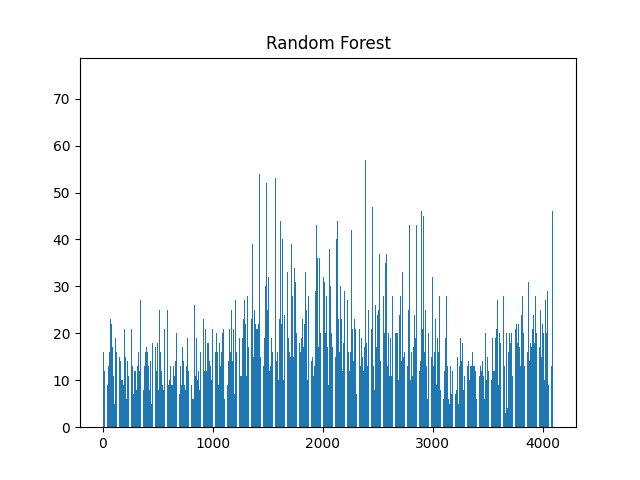
\includegraphics[width=1\linewidth]{1b/Figure_2_bra.png}  
  \caption{Put your sub-caption here}
  \label{RandForSel}
\end{subfigure}
\begin{subfigure}{.33\textwidth}
  \centering
  % include second image
  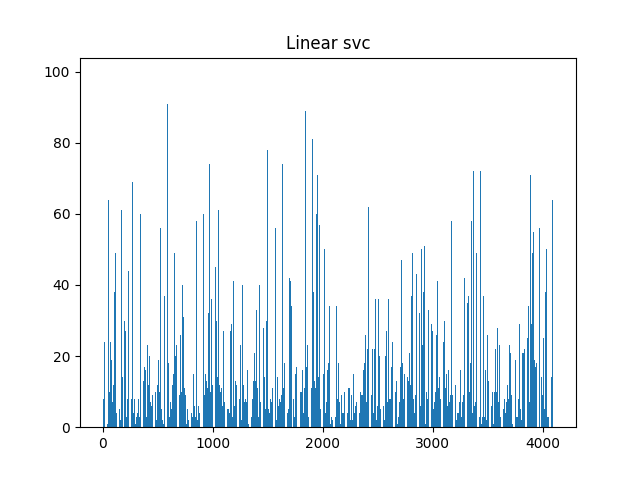
\includegraphics[width=1\linewidth]{1b/Figure_3_bra.png}  
  \caption{Put your sub-caption here}
  \label{fig:sub-second}
\end{subfigure}
\begin{subfigure}{.33\textwidth}
  \centering
  % include second image
  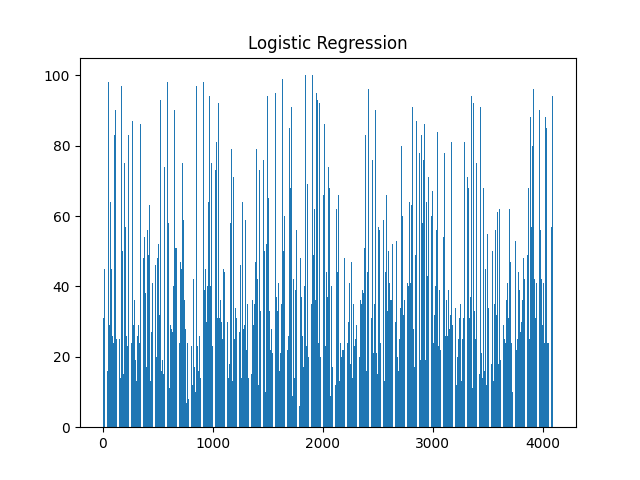
\includegraphics[width=1\linewidth]{1b/Figure_1_bra.png}  
  \caption{Put your sub-caption here}
  \label{fig:sub-second}
\end{subfigure}
\caption{Put your caption here}
\label{imp feat}
\end{figure}

\begin{figure}[ht]
\begin{subfigure}{.33\textwidth}
  \centering
  % include first image
  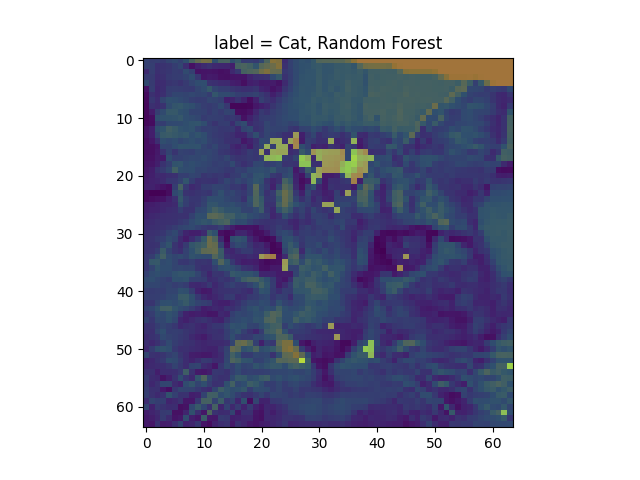
\includegraphics[width=1\linewidth]{1b/Imp_feat RandForest.png}  
  \caption{Put your sub-caption here}
  \label{RandF}
\end{subfigure}
\begin{subfigure}{.33\textwidth}
  \centering
  % include second image
  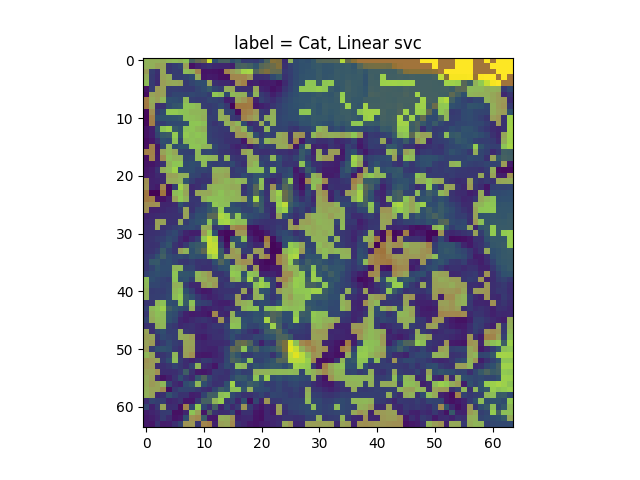
\includegraphics[width=1\linewidth]{1b/Imp_feat_svc.png}  
  \caption{Put your sub-caption here}
  \label{fig:sub-second}
\end{subfigure}
\begin{subfigure}{.33\textwidth}
  \centering
  % include second image
  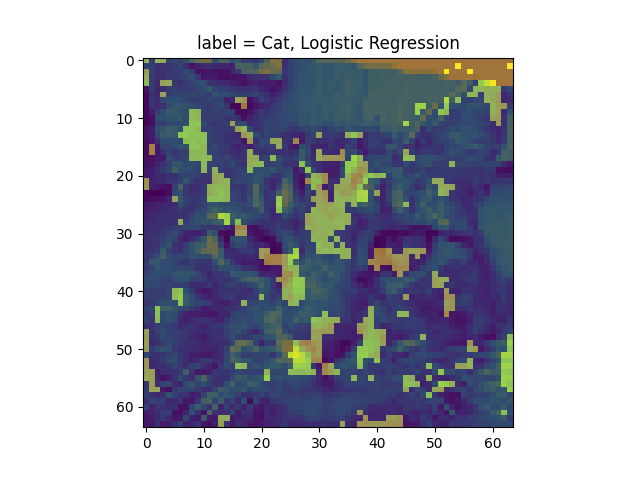
\includegraphics[width=1\linewidth]{1b/Imp_feat LogReg.png}  
  \caption{Put your sub-caption here}
  \label{fig:sub-second}
\end{subfigure}
\caption{Put your caption here}
\label{imp pixels}
\end{figure}
\newpage
\section{c}
\subsection{Result}
The clustering method used was gaussian mixture model and the data was preprocessed by normalization and using principle components. A cutoff at 0.03 was chosen to decide the number of PCA used which is indicated by the red line in figure \ref{scree}. How well the clustering worked was measured by two factors: one how well the clusters agree with the class labels and the Silhouette score. In figure \ref{LabelOverlap} the percentage of dogs in each cluster can be seen for different amount of clusters with the remaining percentage being cats. From the figure one can see that having more than two clusters leads to several clusters having having around 40-60\% of dogs and cats in them which indicates that these clusters don't agree well with the class labels. Moreover the Silhouette score seen in table \ref{sill} seem to suggest that 3 clusters yield the best clustering. However the Silhouette score is low overall which indicates that there is a lot of overlap between the clusters.      

\begin{comment}
\begin{figure}[ht]
\begin{subfigure}{.5\textwidth}
  \centering
  % include first image
  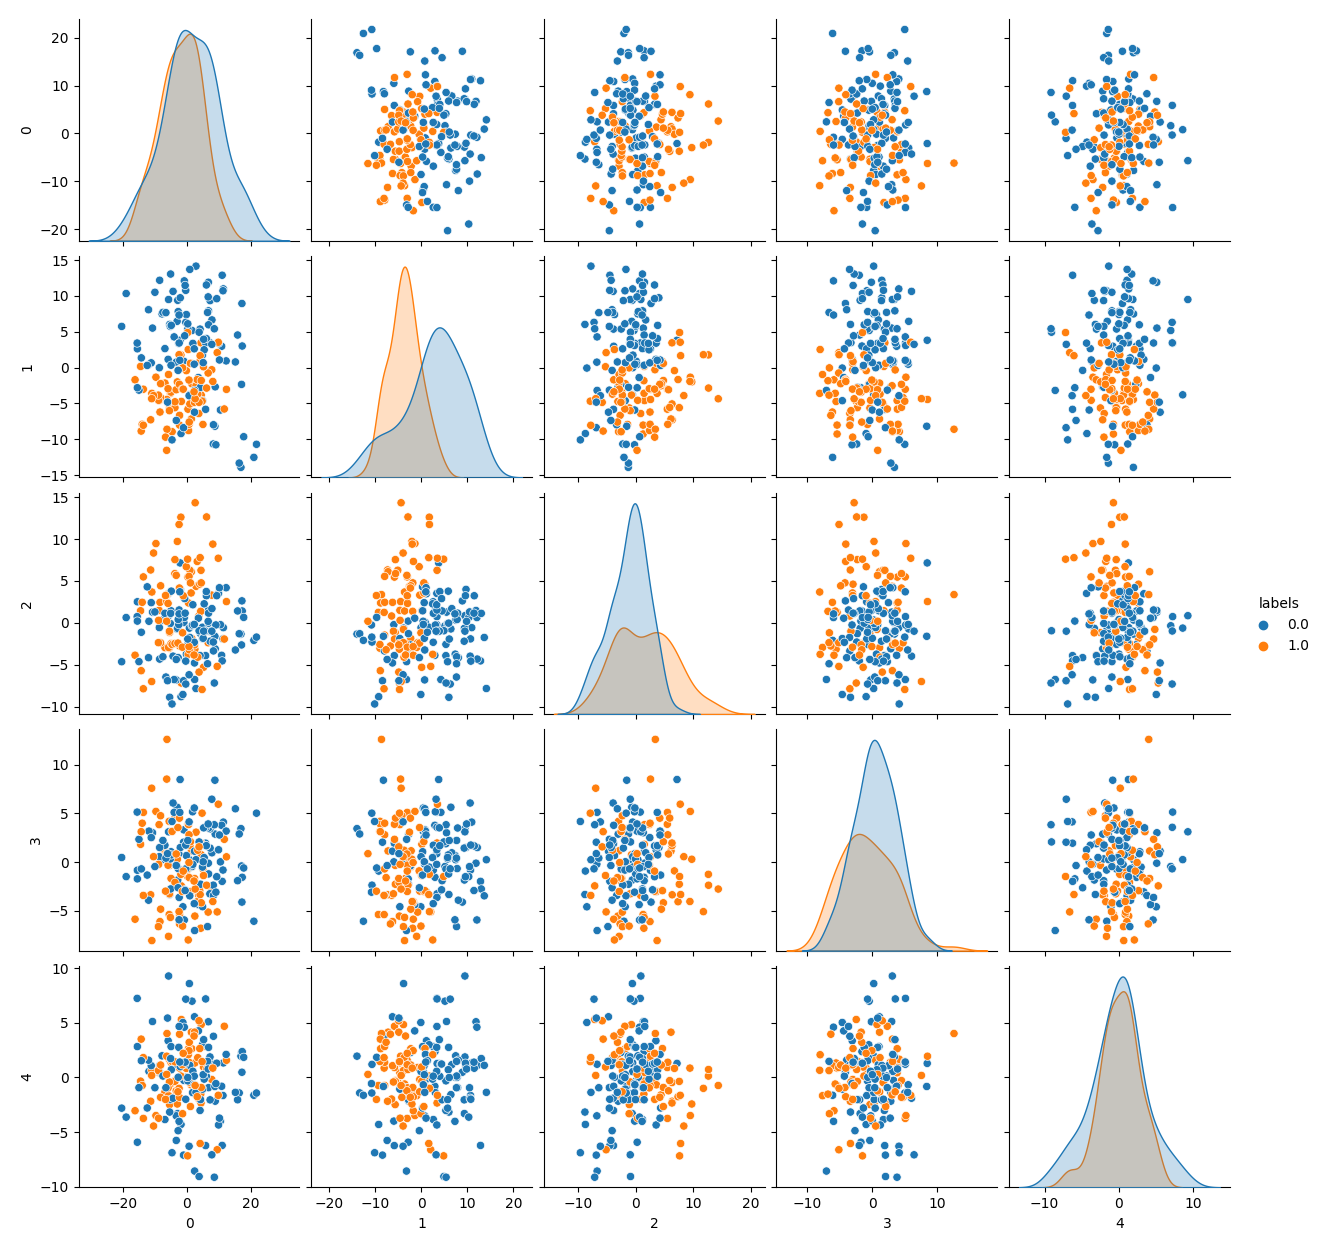
\includegraphics[width=1\linewidth]{1c/True labels sns.png}  
  \caption{Put your sub-caption here}
  \label{fig:sub-first}
\end{subfigure}
\begin{subfigure}{.5\textwidth}
  \centering
  % include second image
  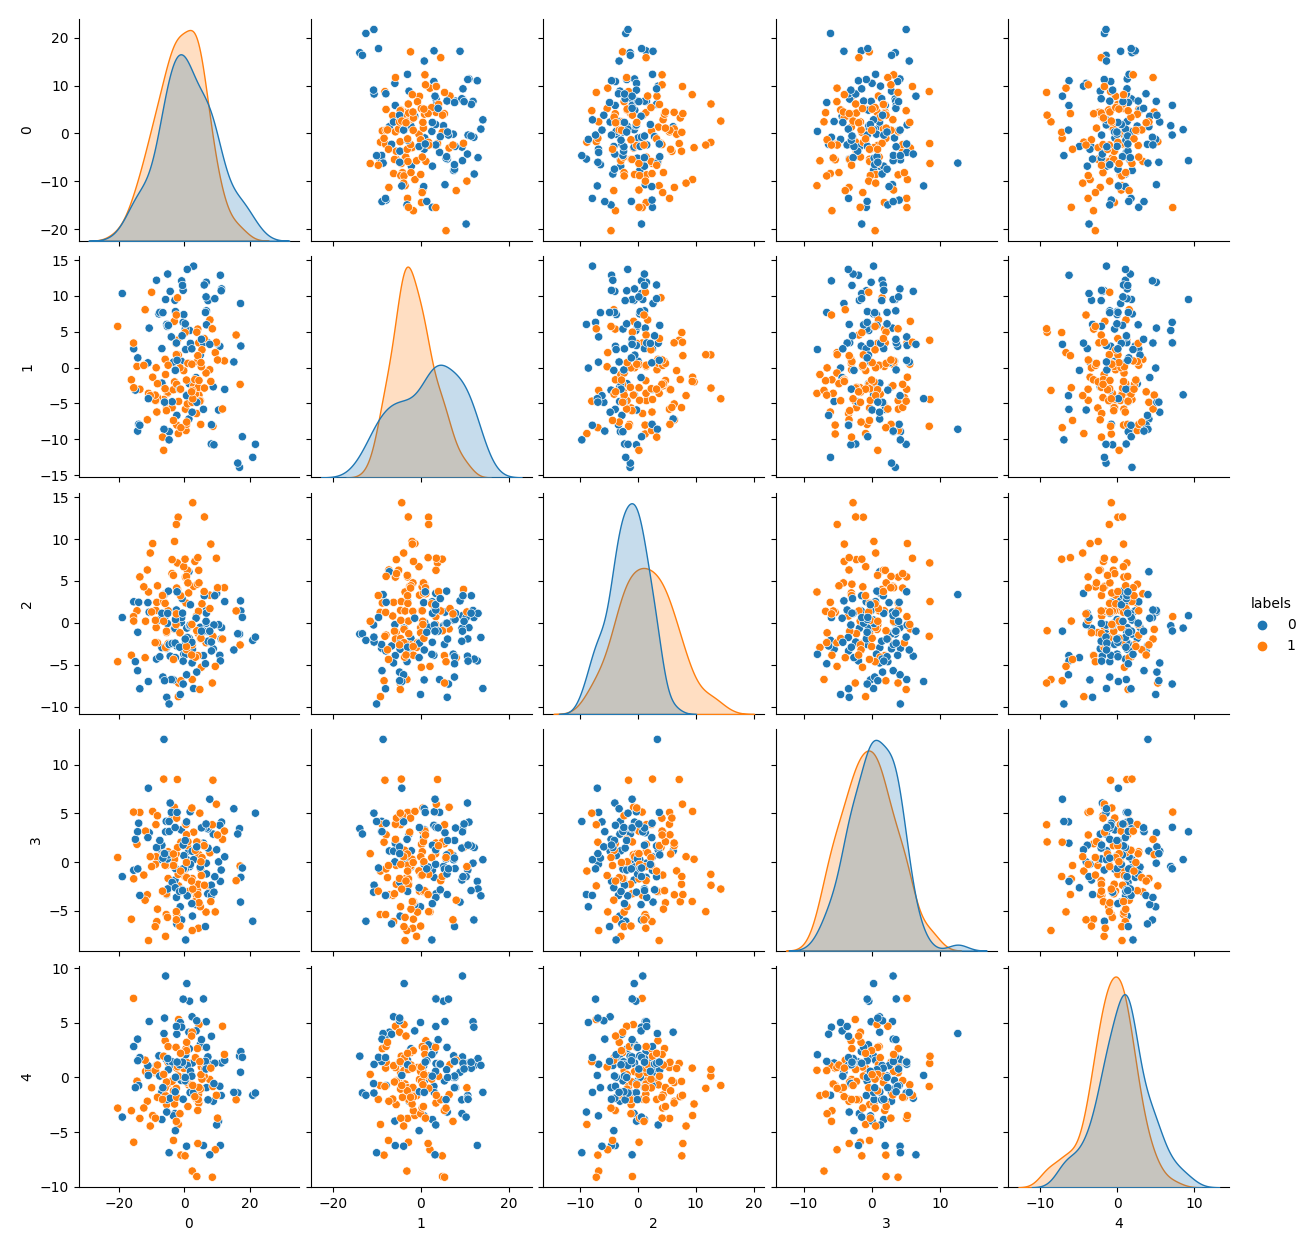
\includegraphics[width=1\linewidth]{1c/two clusters gmm sns.png}  
  \caption{Put your sub-caption here}
  \label{fig:sub-second}
\end{subfigure}
\caption{Put your caption here}
\label{imp pixels}
\end{figure}
\end{comment}
Gaussian mixture model is a method which generally works quite well since it only assumes that the data can be split into normally distributed sub-classes however we can see that it struggles to produce well separated clusters containing only dogs and cats. This could be due to the fact that the cats and dogs data is not well separated which can be seen by looking at the pair plot of the PCA reduced data see figure \ref{pca}. PCA was choosen since we have a high correlation between many of the pixels (features) since it's a picture of an animal if one pixel has a color (rgb value) the ones next to it will in most cases have a similar value. As to which characteristics of the data the clustering picks up a similar feature selection as in 1b was made for the clusters containing most dogs and the one with most cats, for the dogs it seemed like the area around the right ear was the charactersistic picked up by the cluster whilst for the cats the entire right most side of the picture was the most important. It also seemed to be mostly dark cats in the cat majority cluster containing the cats whilst there were mostly brighter pictures in the dog majority cluster.
\subsection{Conclusion}
The clusters don't seem to agree to well with the class labels since no number of clusters produces purely clusters containing only dogs or cats as seen in the example for 2, 3 and 8 clusters in \ref{LabelOverlap}. Furthermore the clusters don't seem to be well spread since the low Silhuette scores seen in \ref{sill} suggests that members in clusters fit well in neighbouring clusters as well. 
\begin{figure}[ht]
\begin{subfigure}{.33\textwidth}
  \centering
  % include first image
  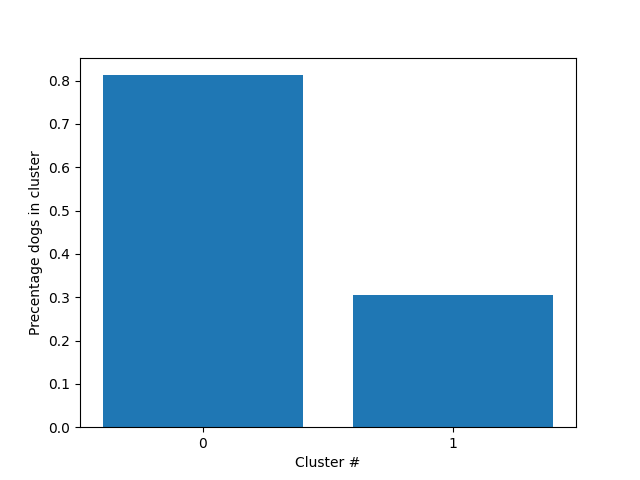
\includegraphics[width=1\linewidth]{1c/label overlapp 2 clusters.png}  
  \caption{Put your sub-caption here}
  \label{fig:sub-first}
\end{subfigure}
\begin{subfigure}{.33\textwidth}
  \centering
  % include second image
  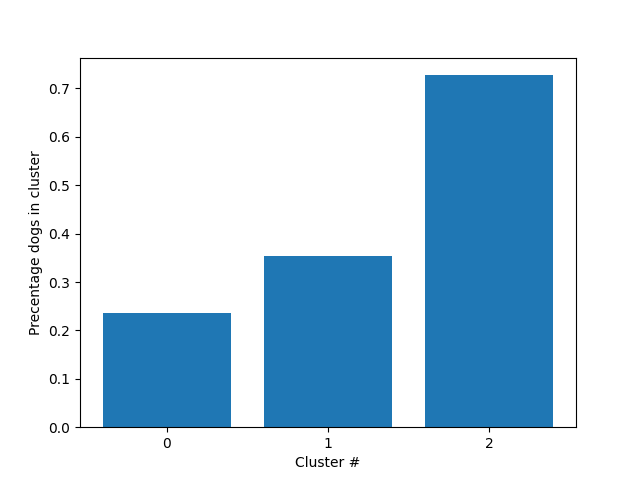
\includegraphics[width=1\linewidth]{1c/label overlapp 3 clusters.png}  
  \caption{Put your sub-caption here}
  \label{fig:sub-second}
\end{subfigure}
\begin{subfigure}{.33\textwidth}
  \centering
  % include second image
  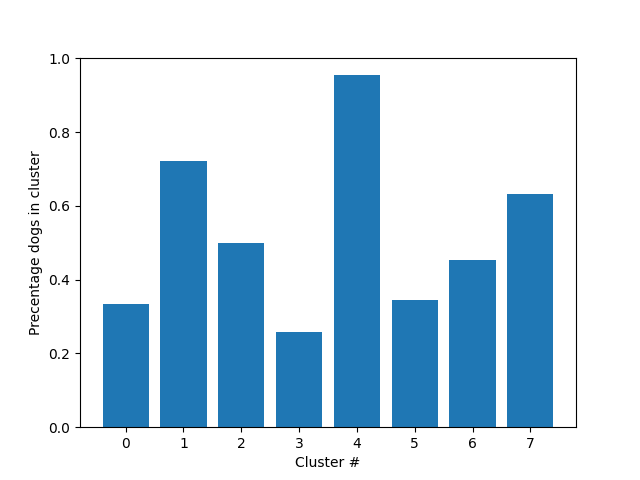
\includegraphics[width=1\linewidth]{1c/label overlapp 8 clusters.png}  
  \caption{Put your sub-caption here}
  \label{fig:sub-second}
\end{subfigure}
\caption{Put your caption here}
\label{LabelOverlap}
\end{figure}
\begin{table}[H]
    \centering
    \begin{tabular}{c|c|c|c|c|c|c|c}
        # clusters & 2& 3& 4& 5& 6& 7& 8  \\
       Silhouette score  & 0.111 & 0.133 & 0.115 & 0.119 &  0.125 &  0.115 &  0.112 \\
       std & 0.026 &  0.027 &  0.027 &  0.026 &  0.021 &  0.027 &  0.025 
    \end{tabular}
    \caption{Caption}
    \label{sill}
\end{table}

\begin{figure}[H]
    \centering
    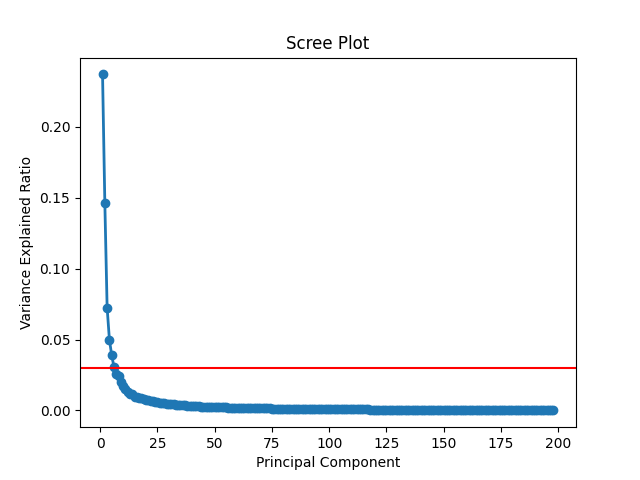
\includegraphics[scale=0.4]{1c/Scree plot.png}
    \caption{Caption}
    \label{scree}
\end{figure}

\begin{figure}[H]
    \centering
    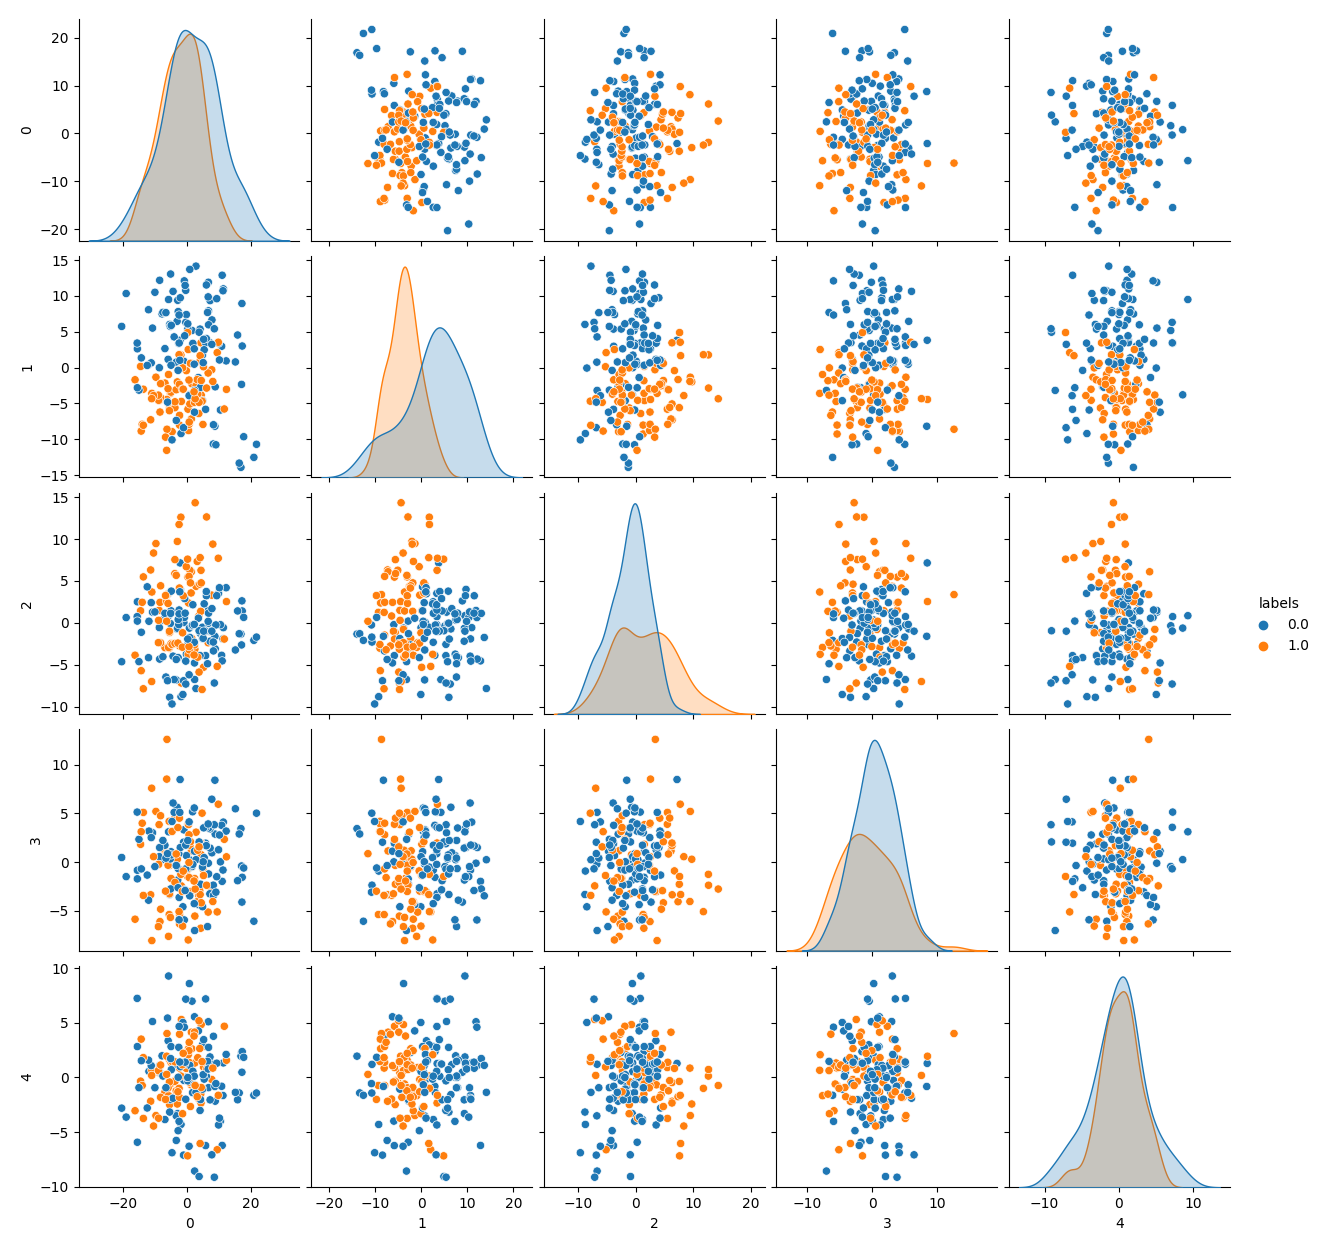
\includegraphics[scale = 0.3]{1c/True labels sns.png}
    \caption{Caption}
    \label{pca}
\end{figure}
%%%%%%%%%%%%%%%%%%%%%%%%%
\newpage
\section{d}
\subsection{Results}
Firstly the data was split into cats and dogs then the same process as in c was made with gmm. However now three internal indices were looked at in order to find the appropriate cluster number for both data sets see figure \ref{Int indiciees} and figure \ref{Int indiciees dog} where the clustering was made for each number of clusters 100 times and the mean value of the internal indices used. As for the Cats based on all three index values shown in \ref{Int indiciees} three clusters would be the best whilst two looks like the best option for the dogs. The reason why there are three clusters of cats whilst only two for dogs could perhaps be explained by the fact that cats have more groups of similar features e.g. if the cats have three distinct colors whilst the dogs mostly only have two. As to which characteristics of the data the different clusters pick up it was difficult to see a clear pattern by looking at the pictures in each cluster see figure \ref{example cat} and figure \ref{example dog}. Except for the difference between cluster 1 and 2 in the cats where it seems like darker cats with brighter background are over represented in cluster one and bright cats with darker background in cluster 2. 
\subsection{Conclusions}
In conclusion the internal indicies suggest that the cats have 3 clusters whilst the dogs have 2, two of the cluster for the cats seem to label the data to the clusters depending on weather the background is dark and the cat bright or vise versa. For the dogs it was difficult to see what features of the picture was classified to each of the clusters.
\begin{figure}[ht]
\begin{subfigure}{.33\textwidth}
  \centering
  % include first image
  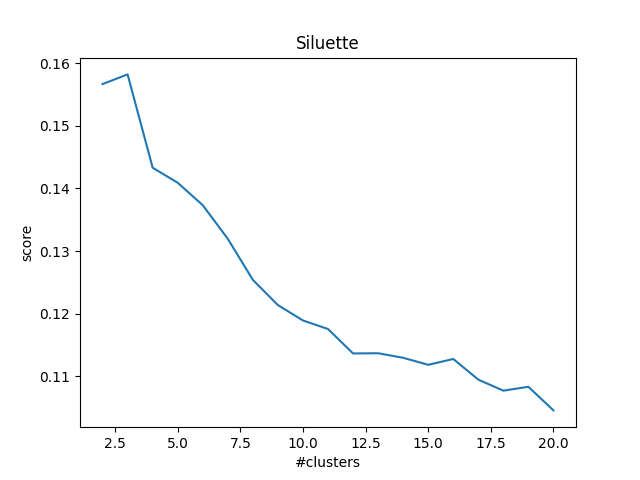
\includegraphics[width=1\linewidth]{1d/Cats/siluette cats.png}  
  \caption{Put your sub-caption here}
  \label{fig:sub-first}
\end{subfigure}
\begin{subfigure}{.33\textwidth}
  \centering
  % include second image
  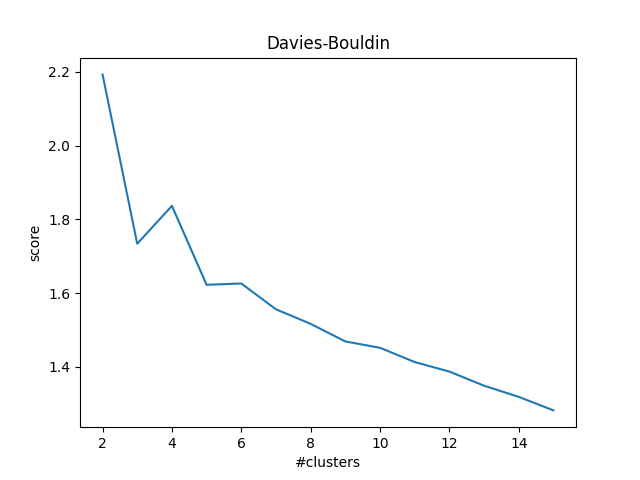
\includegraphics[width=1\linewidth]{1d/Cats/davies cats.png}  
  \caption{Put your sub-caption here}
  \label{fig:sub-second}
\end{subfigure}
\begin{subfigure}{.33\textwidth}
  \centering
  % include second image
  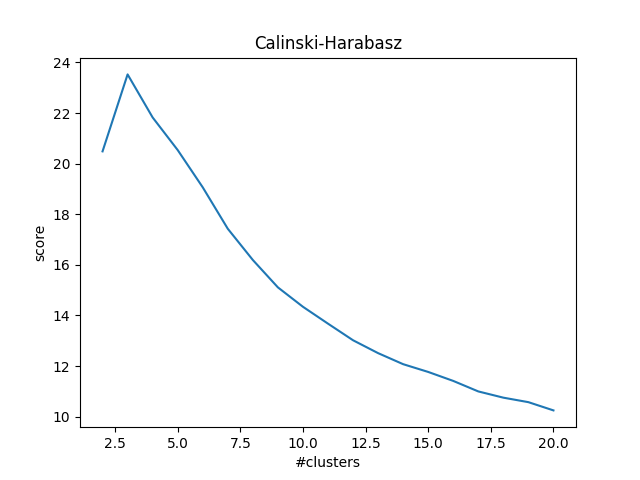
\includegraphics[width=1\linewidth]{1d/Cats/Calinski cats.png}  
  \caption{Put your sub-caption here}
  \label{fig:sub-second}
\end{subfigure}
\caption{Put your caption here}
\label{Int indiciees}
\end{figure}
\begin{figure}[ht]
\begin{subfigure}{.33\textwidth}
  \centering
  % include first image
  \includegraphics[width=1\linewidth]{1d/Dogs/siluette dog.png}  
  \caption{Put your sub-caption here}
  \label{fig:sub-first}
\end{subfigure}
\begin{subfigure}{.33\textwidth}
  \centering
  % include second image
  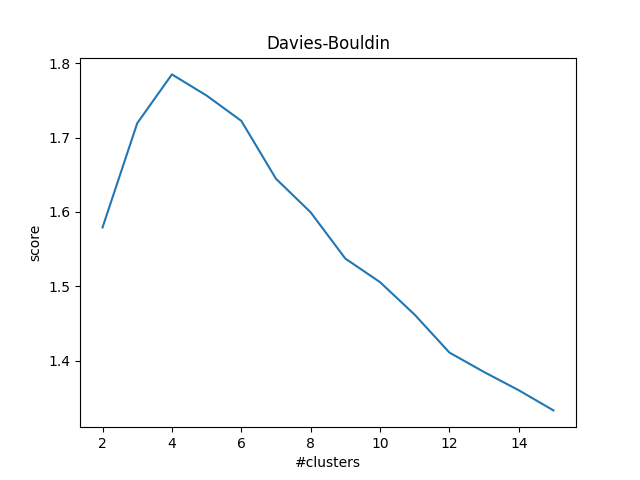
\includegraphics[width=1\linewidth]{1d/Dogs/Davies_dog.png}  
  \caption{Put your sub-caption here}
  \label{fig:sub-second}
\end{subfigure}
\begin{subfigure}{.33\textwidth}
  \centering
  % include second image
  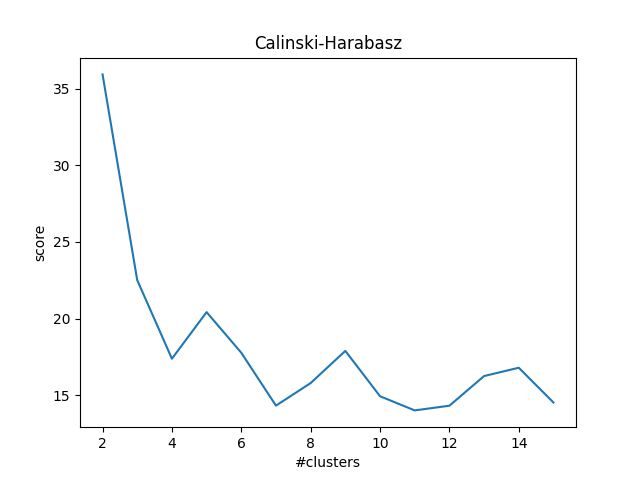
\includegraphics[width=1\linewidth]{1d/Dogs/Calinski dog.png}  
  \caption{Put your sub-caption here}
  \label{fig:sub-second}
\end{subfigure}
\caption{Put your caption here}
\label{Int indiciees dog}
\end{figure}
\begin{figure}[ht]
\begin{subfigure}{.33\textwidth}
  \centering
  % include first image
  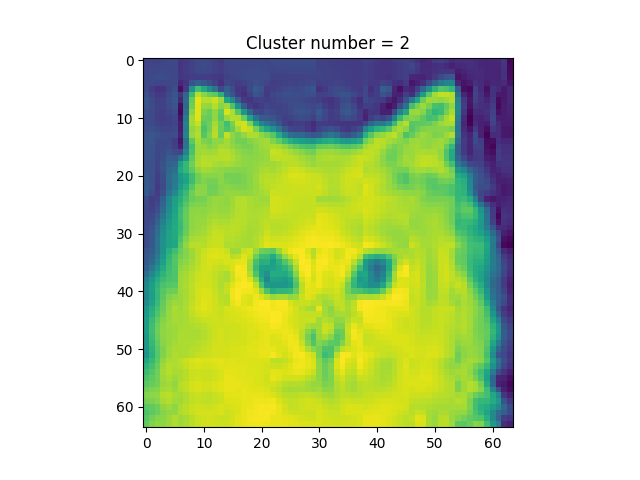
\includegraphics[width=1\linewidth]{1d/Cats/example clust 2.png}  
  \caption{Put your sub-caption here}
  \label{fig:sub-first}
\end{subfigure}
\begin{subfigure}{.33\textwidth}
  \centering
  % include second image
  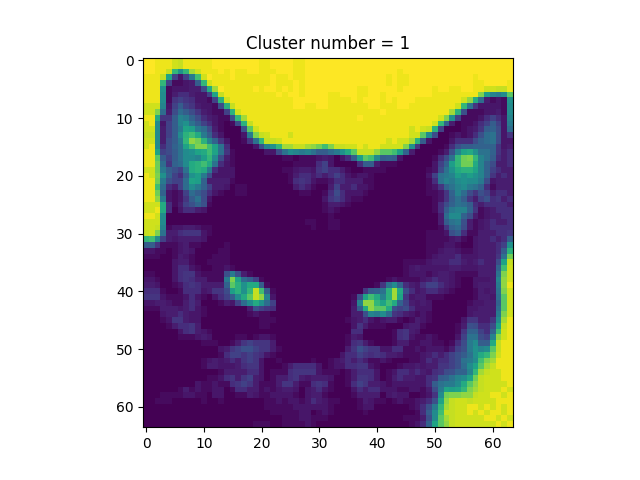
\includegraphics[width=1\linewidth]{1d/Cats/example clust 1.png}  
  \caption{Put your sub-caption here}
  \label{fig:sub-second}
\end{subfigure}
\begin{subfigure}{.33\textwidth}
  \centering
  % include second image
  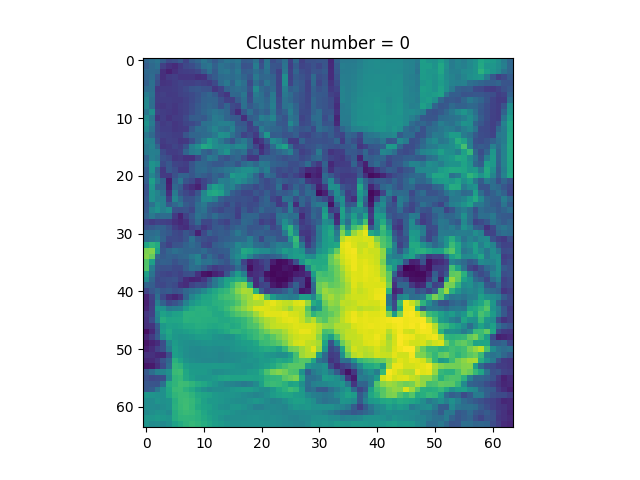
\includegraphics[width=1\linewidth]{1d/Cats/Example clust 0.png}  
  \caption{Put your sub-caption here}
  \label{fig:sub-second}
\end{subfigure}
\caption{Put your caption here}
\label{example cat}
\end{figure}

\begin{figure}[H]
\begin{subfigure}{.33\textwidth}
  \centering
  % include first image
  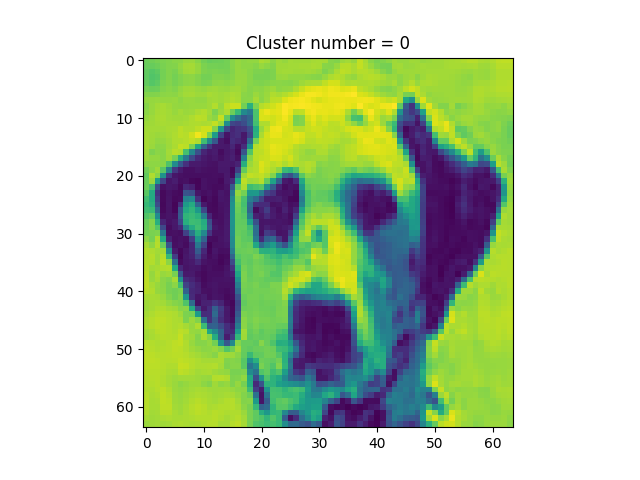
\includegraphics[width=1\linewidth]{1d/Dogs/Example dog clust 1.png}  
  \caption{Put your sub-caption here}
  \label{fig:sub-first}
\end{subfigure}
\begin{subfigure}{.33\textwidth}
  \centering
  % include second image
  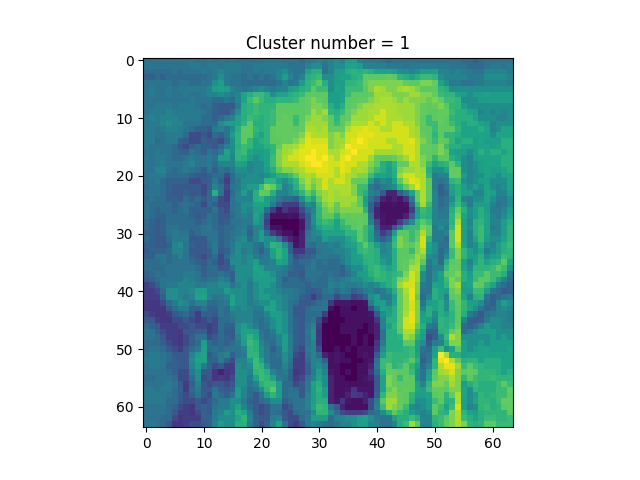
\includegraphics[width=1\linewidth]{1d/Dogs/Example dog clust 0.png}  
  \caption{Put your sub-caption here}
  \label{fig:sub-second}
\end{subfigure}
\caption{Put your caption here}
\label{example dog}
\end{figure}
\newpage
\section{e}
\subsection{Results}
The dogs were clustered into two clusters and the cats into three based on the results from d. The same bootstrapping method  and classifyers used in b was then implemented for finding the important features for each classifier. Since we now are classifying only dogs and cats separately there should be different features which are of importance compared to b. The reasoning behind this is that the different types of dogs have different pixels which separates them from each other than the ones important for separating dogs from cats, the same goes for the cats. Looking at figures \ref{LogReg dog} and \ref{LogReg cat} one can see that the features which the logistic regression deems important follows the outlines of the cats and dogs and seems to look at most parts of the pictures for classifying them to a certain cluster. The Ranbdom Forest algorithm seems to look at very specific pixels for the dogs data set with only a couple of pixels being selected over 80\% during the bootstrapping see figure \ref{rndf selection}. This differs from the results in b and the one for the cats see figure \ref{rndf selection cat} where the feature selection isn't as confident on which pixels to choose. This could be due to the fact that larger groups of highly correlated features are given lesser relevance than smaller ones in the random forest algorithm and since we are looking at a picture it's not unreasonable to assume that there are large clusters of pixels with high correlation. As for the linear SVM model the model seems to select features around the right ear and nose with confidence see figures \ref{svc selection} and \ref{linear svc selection cat}. The reeason the Svm with linear kernal dosen't select featrures following the structure of the dog aswell as the logistic regression could be due to the fact that using a hyperplane to seperate cats from cats or dogs from dogs is a poor idea so this could be an effect of the linear kernal used. 
\subsection{Conclusions}
In conclusion it's clear that the logistic regression looks at many parts of the picture and has high confidence in a lot of its feature selections whilst the Random Forrest behaves differently and has a few pixels with high confidence which it deems important whilst the linear svm model selects roughly around the eyes right ear and nose however the selected features aren't very neatly clustered around certain areas so it's difficult to see exactly what parts of the animal it deems important for classification. 
\begin{figure}[H]
\begin{subfigure}{.33\textwidth}
  \centering
  % include first image
  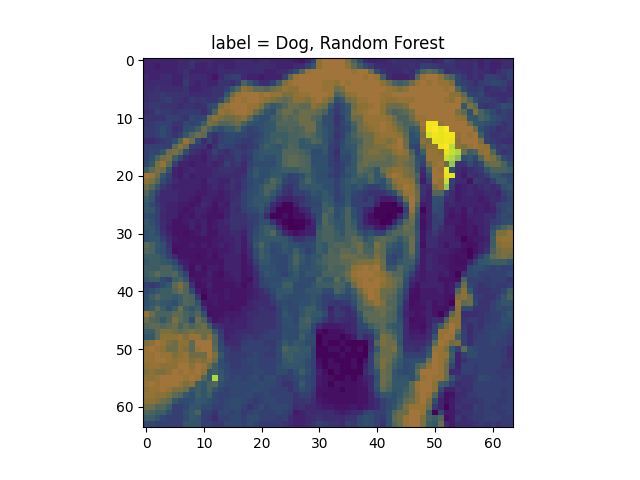
\includegraphics[width=1\linewidth]{1e/Dogs 2 clusters/imp feat RandomForest pic.png}  
  \caption{Put your sub-caption here}
  \label{rndf selection}
\end{subfigure}
\begin{subfigure}{.33\textwidth}
  \centering
  % include second image
  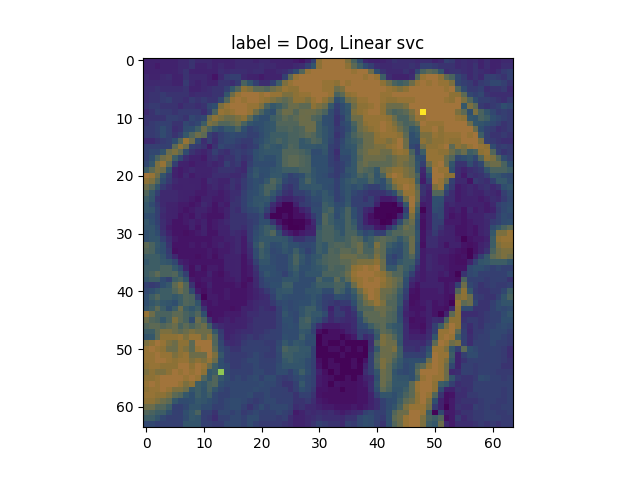
\includegraphics[width=1\linewidth]{1e/Dogs 2 clusters/imp_feat Linear svc.png}  
  \caption{Put your sub-caption here}
  \label{}
\end{subfigure}
\begin{subfigure}{.33\textwidth}
  \centering
  % include second image
  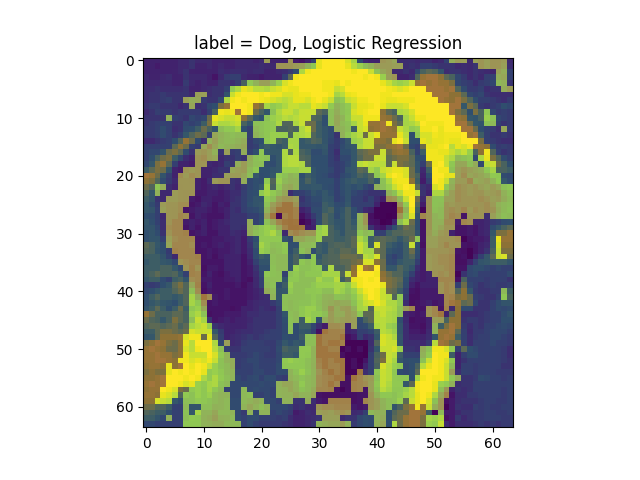
\includegraphics[width=1\linewidth]{1e/Dogs 2 clusters/imp feat LogisticRegression.png}  
  \caption{Put your sub-caption here}
  \label{LogReg dog}
\end{subfigure}
\caption{Put your caption here}
\label{example dog}
\end{figure}
\begin{figure}[H]
\begin{subfigure}{.33\textwidth}
  \centering
  % include first image
  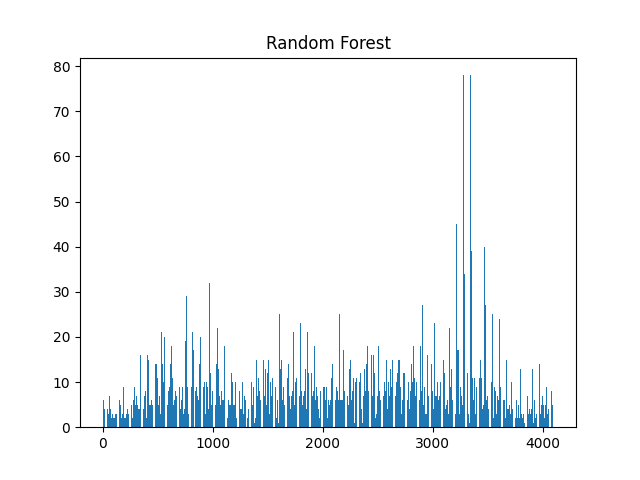
\includegraphics[width=1\linewidth]{1e/Dogs 2 clusters/selection Random Forest.png}  
  \caption{Put your sub-caption here}
  \label{fig:sub-first}
\end{subfigure}
\begin{subfigure}{.33\textwidth}
  \centering
  % include second image
  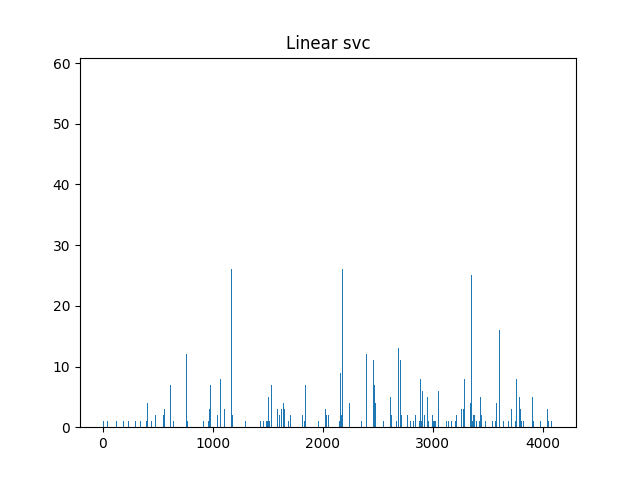
\includegraphics[width=1\linewidth]{1e/Dogs 2 clusters/selection linear svc.png}  
  \caption{Put your sub-caption here}
  \label{svc selection}
\end{subfigure}
\begin{subfigure}{.33\textwidth}
  \centering
  % include second image
  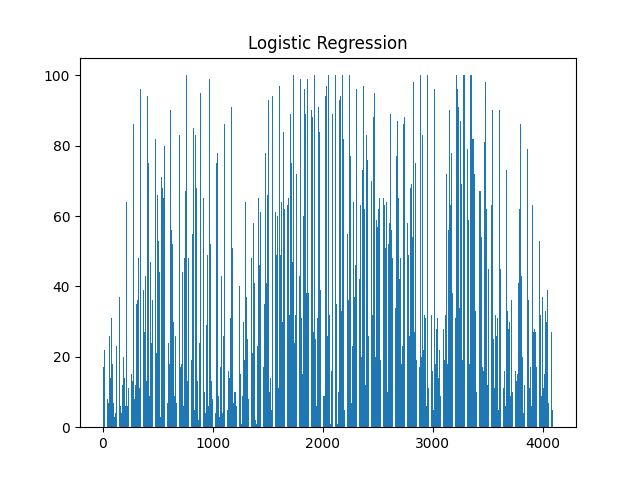
\includegraphics[width=1\linewidth]{1e/Dogs 2 clusters/selection Logistic.png}  
  \caption{Put your sub-caption here}
  \label{fig:sub-second}
\end{subfigure}
\caption{Put your caption here}
\label{example dog}
\end{figure}

\begin{figure}[H]
\begin{subfigure}{.33\textwidth}
  \centering
  % include first image
  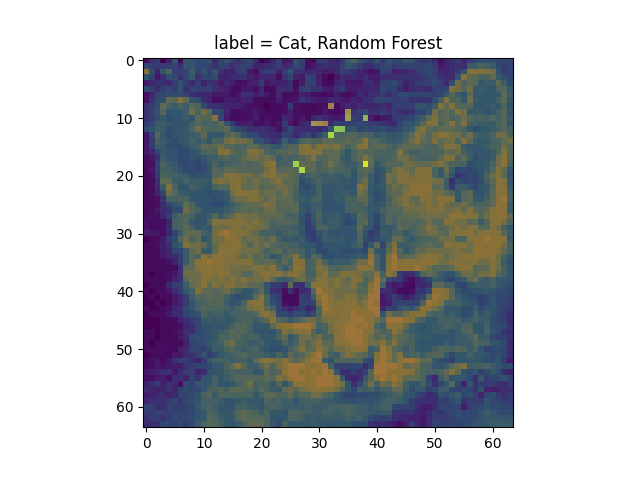
\includegraphics[width=1\linewidth]{1e/Cats 5 clusters/impfeat RandomForest.png}  
  \caption{Put your sub-caption here}
  \label{}
\end{subfigure}
\begin{subfigure}{.33\textwidth}
  \centering
  % include second image
  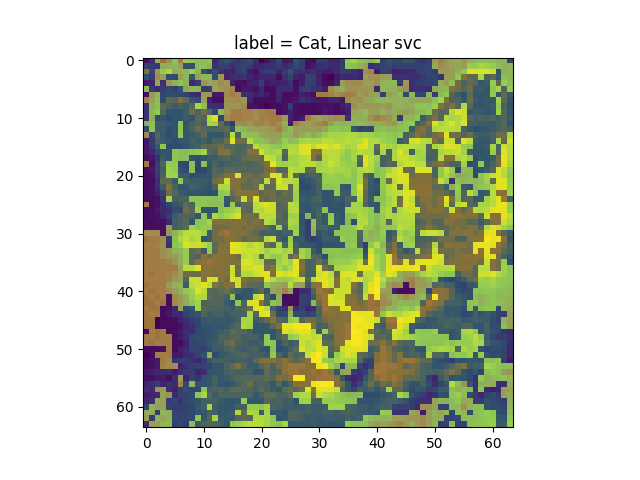
\includegraphics[width=1\linewidth]{1e/Cats 5 clusters/impfeat linear svc bra.png}  
  \caption{Put your sub-caption here}
  \label{fig:sub-second}
\end{subfigure}
\begin{subfigure}{.33\textwidth}
  \centering
  % include second image
  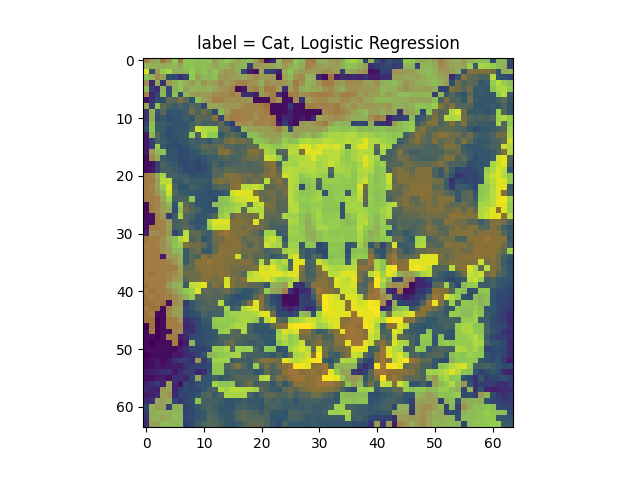
\includegraphics[width=1\linewidth]{1e/Cats 5 clusters/impfeat LogReg.png}  
  \caption{Put your sub-caption here}
  \label{LogReg cat}
\end{subfigure}
\caption{Put your caption here}
\label{example dog}
\end{figure}
\begin{figure}[H]
\begin{subfigure}{.33\textwidth}
  \centering
  % include first image
  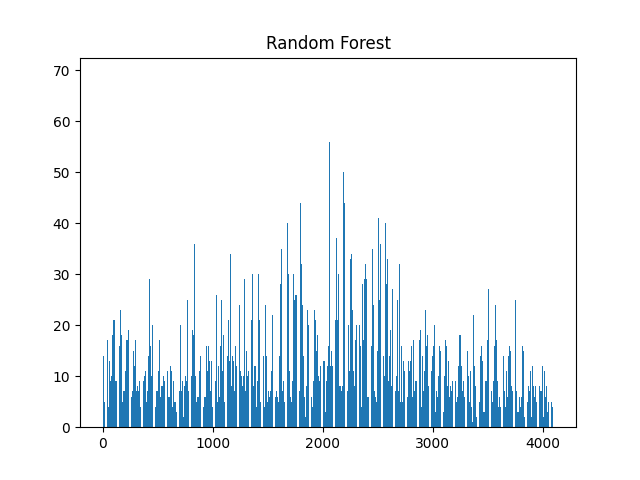
\includegraphics[width=1\linewidth]{1e/Cats 5 clusters/selected RandomForest.png}  
  \caption{Put your sub-caption here}
  \label{rndf selection cat}
\end{subfigure}
\begin{subfigure}{.33\textwidth}
  \centering
  % include second image
  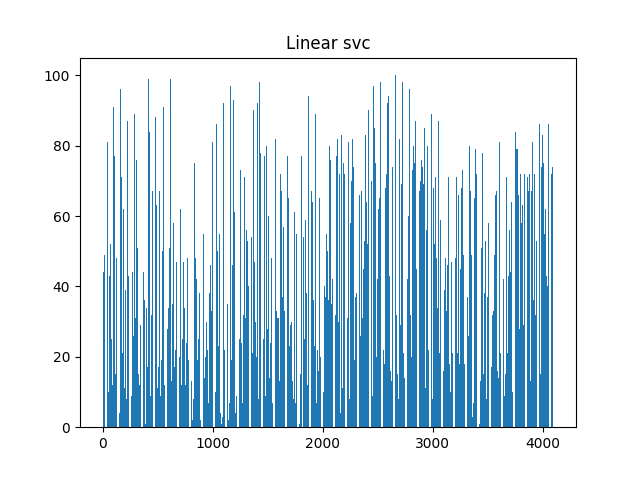
\includegraphics[width=1\linewidth]{1e/Cats 5 clusters/selected LinearSvc.png}  
  \caption{Put your sub-caption here}
  \label{linear svc selection cat}
\end{subfigure}
\begin{subfigure}{.33\textwidth}
  \centering
  % include second image
  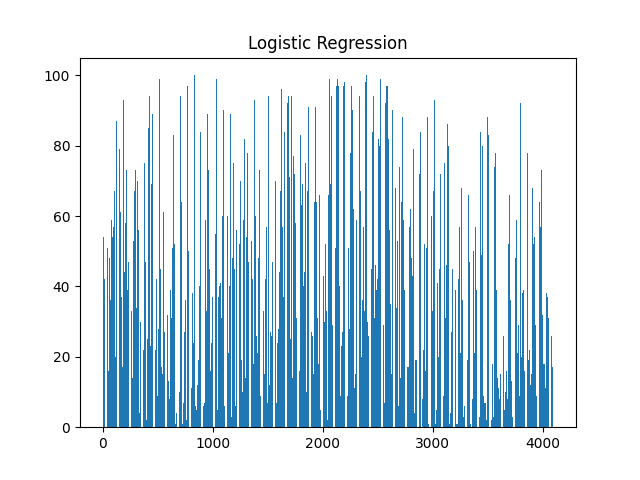
\includegraphics[width=1\linewidth]{1e/Cats 5 clusters/selected LogReg.png}  
  \caption{Put your sub-caption here}
  \label{fig:sub-second}
\end{subfigure}
\caption{Put your caption here}
\label{example dog}
\end{figure}

\newpage
\section{f}
\subsection{Results}
The data was firstly split into a subset of cats and the rest as test data the same procedures as in c with PCA was then made see figure \ref{scree 1f}. A logistic regression model was then fitted to the data set, it was difficult to tune the hyper parameter this time around since the data set to cross validate contained so few data points which could effect  the performance of the classifier. The classifier was then ran on the test data set and classified all data points to the cluster labels. In order to see weather it could separate the dogs from the cats the precentage of dogs in each cluster was recored see figure \ref{1f}. When the result was averaged over 100 runs as seen in the left most graph the classifier could not separate the dogs from cats. However during some single runs there would be clusters of data containing mostly dogs and the rest none as seen in the right most picture in figure \ref{1f}. 
\subsection{Conclusions}
It doesn't seem like the classification method can separate dogs from cats by looking at the clustered subset of cats. However during some runs it would separate cats from dogs very well this could be an effect of which data was chosen in the subset of cats where if images of cats with doglike features were in the clustered data set perhaps the classifier could learn to separate the dogs from cats. It could also be an effect of the miss labeled data being selected in the cat subset since if enough of them were selected one cluster could have an majority of dogs which were labeled as cats.  
\begin{figure}[H]
\begin{subfigure}{.5\textwidth}
  \centering
  % include first image
  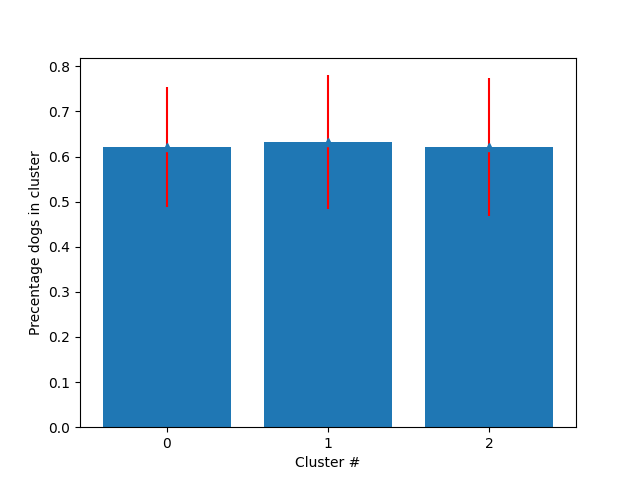
\includegraphics[width=1\linewidth]{1f/clustering avg.png}  
  \label{1fa}
\end{subfigure}
\begin{subfigure}{.5\textwidth}
  \centering
  % include second image
  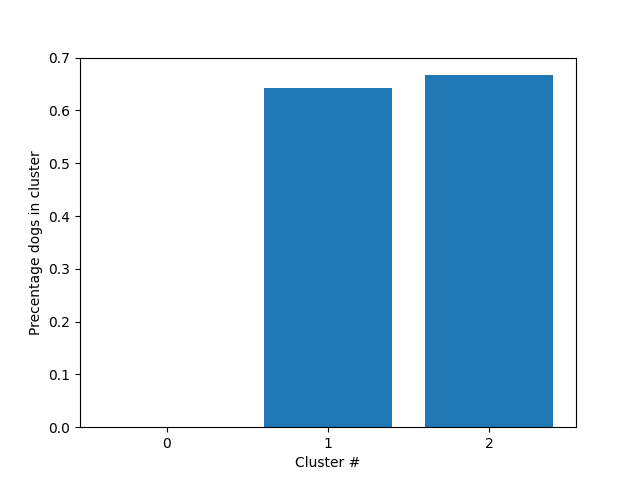
\includegraphics[width=1\linewidth]{1f/clustering.png}  
  \label{1f b}
\end{subfigure}
\caption{Put your caption here}
\label{1f}
\end{figure}
\begin{figure}[H]
    \centering
    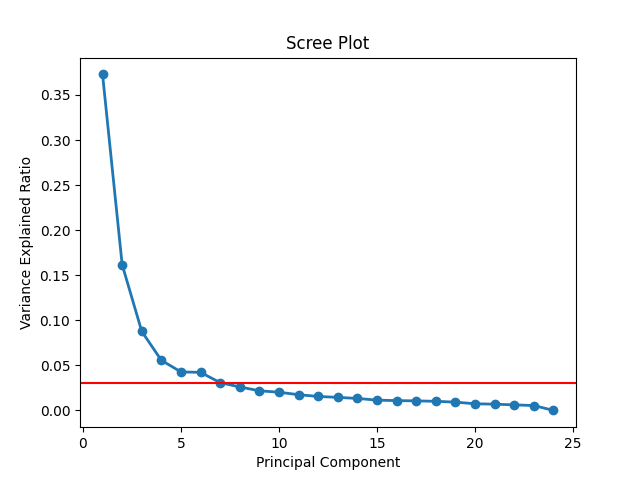
\includegraphics[scale=0.5]{1f/Scree.png}
    \caption{Caption}
    \label{scree 1f}
\end{figure}
\end{document}